\chapter{Iteración 1}

\begin{quotation}[Philosopher]{Lao Tzu (c. 6th century BC)}
The journey of a thousand miles begins with one step.
\end{quotation}

\begin{abstract}
Esta iteración abre la parte de ejecución, seguimiento y control de la memoria. A partir
de este punto, el desarrollo se documenta mediante iteraciones cerradas que recogen las
funcionalidades trabajadas, las decisiones de diseño, la implementación realizada y su
validación posterior. En concreto, esta primera iteración establece la base jugable
mínima del proyecto mediante la generación procedural del mapa, la incorporación del
jugador y la activación inicial de enemigos dentro de las salas.
\end{abstract}

\section{Lista de funcionalidades}
La primera iteración se concibió como la primera entrega jugable del proyecto. Hasta este
momento existía una base conceptual clara, pero todavía no se había construido un ciclo de
juego verificable dentro del motor. Por ello, el objetivo de esta iteración fue establecer
el núcleo mínimo que permitiera comprobar si la dirección técnica elegida era viable:
generar un nivel, instanciarlo en escena, introducir una entidad controlable y poblar las
salas con enemigos básicos.

Siguiendo el enfoque de \textit{Feature Driven Development} (FDD), en esta iteración se
abordaron tres funcionalidades que definen el arranque real del sistema:

\begin{enumerate}
\item \textbf{Generación Procedural.} Esta funcionalidad introdujo el sistema encargado de
crear automáticamente la estructura de la partida cada vez que comienza una \textit{run}.
Su comportamiento real no se limitaba a elegir salas aleatorias, sino a construir una
mazmorra navegable a partir de una rejilla lógica, garantizando que las habitaciones
quedaran conectadas entre sí y que existiese una progresión espacial coherente desde la
sala inicial hacia el resto del nivel. Dentro de esta feature también se incorporó el
soporte para habitaciones de distintas formas y tamaños, evitando que la topología del mapa
quedara reducida a una colección uniforme de salas idénticas. Además, se dejó integrada la
distribución de salas especiales, de modo que el sistema no solo generara espacio, sino que
empezara a diferenciar tipos de habitación con funciones distintas dentro de la partida.
En términos jugables, esta feature es la que hace posible que cada intento tenga una
disposición diferente sin perder coherencia estructural.

\begin{figure}[H]
\begin{center}
\missingfigure{Sustituir por captura representativa de Generación Procedural en la iteración 1}
% \includegraphics[width=.9\textwidth]{figures/iteracion1_generacion_procedural.png}
\caption{Resultado visual de la feature Generación Procedural en la iteración 1}
\label{fig:iteracion1-feature-generacion}
\end{center}
\end{figure}

\item \textbf{Añadir Jugador.} Esta funcionalidad convirtió por primera vez el nivel
generado en un espacio realmente jugable. Su alcance real consistió en incorporar una
entidad controlable capaz de aparecer en la sala inicial de la mazmorra, desplazarse por
las habitaciones instanciadas y servir como punto de referencia para validar colisiones,
escala del escenario y flujo de navegación entre salas. La feature no perseguía todavía un
sistema de acciones complejo, sino confirmar que el personaje podía habitar correctamente
el mapa procedural y recorrerlo con naturalidad dentro del motor. También actuó como base
para el resto de sistemas, ya que la cámara, la activación de salas y el comportamiento de
los enemigos pasan a organizarse en torno a la posición del jugador. En otras palabras, no
era solo ``añadir un personaje'', sino introducir el elemento central a partir del cual la
partida puede empezar a ejecutarse de forma interactiva.

\begin{figure}[H]
\begin{center}
\missingfigure{Sustituir por captura representativa de Añadir Jugador en la iteración 1}
% \includegraphics[width=.9\textwidth]{figures/iteracion1_jugador.png}
\caption{Resultado visual de la feature Añadir Jugador en la iteración 1}
\label{fig:iteracion1-feature-jugador}
\end{center}
\end{figure}

\item \textbf{Añadir Enemigos.} Esta funcionalidad incorporó oposición activa dentro del
nivel y transformó la exploración en una experiencia jugable con tensión y resolución. Su
comportamiento real consistió en poblar determinadas salas con enemigos básicos capaces de
instanciarse correctamente dentro del espacio disponible, detectar al jugador cuando este
entraba en su radio de acción y reaccionar mediante un patrón elemental de persecución y
ataque. La feature también introdujo el vínculo entre enemigos y estado de la sala: al
entrar en una habitación con enemigos, las puertas se cierran temporalmente y el jugador
debe derrotarlos para recuperar el paso. Gracias a ello, cada sala deja de ser un simple
espacio de tránsito y pasa a comportarse como una unidad de encuentro con inicio, bloqueo y
resolución. Esta funcionalidad fue clave para cerrar el primer bucle jugable completo del
proyecto.

\begin{figure}[H]
\begin{center}
\missingfigure{Sustituir por captura representativa de Añadir Enemigos en la iteración 1}
% \includegraphics[width=.9\textwidth]{figures/iteracion1_enemigos.png}
\caption{Resultado visual de la feature Añadir Enemigos en la iteración 1}
\label{fig:iteracion1-feature-enemigos}
\end{center}
\end{figure}
\end{enumerate}

La combinación de estas tres funcionalidades permitió pasar de una base técnica aislada a
una primera versión del bucle jugable: generar un nivel, recorrerlo con el jugador y
resolver encuentros en salas con enemigos. Esta iteración no buscaba todavía profundidad
de contenido ni pulido visual, sino validar que los cimientos arquitectónicos del juego
podían sostener el desarrollo posterior.

\section{Diseño}
Desde el punto de vista del diseño, la iteración se estructuró en torno a tres bloques
coordinados: la generación abstracta del mapa, la materialización de ese mapa en salas
jugables y la interacción de entidades dinámicas dentro de dichas salas. La decisión
principal fue no resolver todo en un único componente central, sino separar las
responsabilidades desde el principio para evitar un crecimiento descontrolado del código.

\subsection{Diseño de la generación procedural}
La generación procedural se apoyó en una rejilla lógica bidimensional. Esta decisión
permitía expresar con claridad las reglas de vecindad, ocupación, expansión y validación
espacial, reduciendo la complejidad del algoritmo respecto a una representación continua.

Sobre esa rejilla se definió una doble lectura del nivel. Por un lado, un modelo espacial,
encargado de saber qué posiciones estaban ocupadas. Por otro, un modelo lógico, centrado
en las relaciones entre habitaciones y en la navegabilidad general del mapa. Esta
separación fue importante porque permitía pensar la topología de la mazmorra sin acoplarla
directamente a su representación visual.

Además, desde esta primera iteración se contempló que no todas las habitaciones debían ser
de tamaño unitario. Se decidió soportar salas de 1x1, 1x2, 2x1, 2x2 y con forma de L, ya
que limitar la generación a salas idénticas habría simplificado el arranque, pero también
habría empobrecido mucho la expresividad espacial del sistema.

\subsection{Diseño de la instanciación de salas}
Una vez generada la topología abstracta del nivel, era necesario traducirla a una escena
jugable dentro de Unity. Para ello se separó la responsabilidad del generador de mapa de la
responsabilidad de instanciar salas concretas. El generador produce la descripción lógica
del nivel; el gestor de salas decide cómo materializar esa descripción.

Cada sala se diseñó como una unidad autocontenida responsable de su variación visual, sus
puertas, sus muros y las entidades que aloja. Esta decisión hacía que el comportamiento de
una habitación pudiera encapsularse localmente y reducía el acoplamiento con el resto del
sistema.

\subsection{Diseño del jugador y de los enemigos}
El jugador se diseñó inicialmente con un enfoque deliberadamente simple. La prioridad era
validar movimiento, navegación y lectura del espacio antes de introducir mecánicas más
complejas. Por ello, el diseño se apoyó en un controlador de desplazamiento básico,
suficiente para recorrer el nivel generado y comprobar la coherencia del mapa.

Los enemigos también se diseñaron con una estructura mínima pero extensible. En lugar de
implementar desde el principio un sistema de IA complejo, se definió una máquina de estados
elemental con tres comportamientos: reposo, persecución y ataque. Esta decisión permitía
introducir oposición funcional sin comprometer la estabilidad del arranque.

Por último, se decidió que la sala, y no el enemigo individual, fuese la responsable del
ritmo general del encuentro. Así, al entrar por primera vez en una habitación con enemigos,
la propia sala podía bloquear las puertas y liberarlas cuando el combate hubiese terminado.

\section{Implementación}
La implementación de esta iteración se realizó siguiendo el mismo orden lógico en el que se
habían diseñado las features: primero la estructura del mundo, después la integración del
jugador y, finalmente, la incorporación de enemigos y control de encuentros.

\subsection{Implementación de la generación procedural}
La construcción del mapa partió de una estructura de ocupación y de una estrategia de
expansión controlada hacia celdas adyacentes. El algoritmo arranca desde una posición
central y explora posiciones vecinas siempre que se cumplan ciertas restricciones:
disponibilidad espacial, límite de habitaciones y validez estructural de la expansión.

Una vez aceptada una nueva posición, el sistema decide si se trata de una sala simple o de
una sala compuesta por varias celdas. A continuación se registra tanto su ocupación física
como su papel dentro de la estructura lógica del nivel. Esta fase permitió construir mapas
con variedad geométrica sin perder el control sobre la navegabilidad.

Tras generar el trazado principal, se asignaron las salas especiales. Aunque en esta
iteración todavía no se explotaban todas sus posibilidades jugables, dejarlas integradas en
la generación resultaba clave para no tener que rediseñar la topología del sistema en fases
posteriores.

\subsection{Implementación de la instanciación de salas}
Con la topología ya disponible, el sistema recorrió las habitaciones generadas y buscó para
cada una una definición visual compatible con su forma y tipo. A partir de esa información
se instanciaron las salas jugables dentro de la escena, ajustando sus dimensiones y
determinando en qué bordes debían colocarse puertas o muros.

Esta fase era especialmente importante porque actuaba como puente entre la lógica abstracta
del generador y el espacio real con el que interactuarían el jugador y los enemigos. Si
esta traducción fallaba, el mapa podía ser correcto desde el punto de vista lógico pero no
jugable en el motor.

\subsection{Implementación del jugador}
El jugador se integró mediante un controlador ligero apoyado en \texttt{Rigidbody2D}. En
cada ciclo se leían las entradas de movimiento y se trasladaban al cuerpo físico del
personaje, obteniendo así una solución suficiente para validar navegación, colisiones y
escala de desplazamiento.

La aparición del jugador se vinculó además a la sala inicial del nivel generado, evitando
depender de una coordenada fija de escena. Esta decisión reforzaba el acoplamiento correcto
entre generación procedural y sistemas jugables, ya que el personaje debía situarse siempre
en una posición coherente con la partida recién creada.

\subsection{Implementación de enemigos y encuentros}
Los enemigos se instanciaron desde las propias salas una vez configuradas. Cada sala
conservaba la referencia a sus enemigos activos, lo que hacía posible asociar el estado del
combate con el estado de la habitación.

El comportamiento de los enemigos se resolvió con una máquina de estados simple basada en
distancia al jugador. Mientras este permanecía fuera de alcance, el enemigo se mantenía en
reposo; cuando entraba en su radio de detección, pasaba a perseguirlo; y al acercarse lo
suficiente, ejecutaba su ataque.

Sobre esa base se añadió el cierre y apertura de puertas como mecanismo de control del
encuentro. Cuando el jugador entraba por primera vez en una sala con enemigos, las puertas
se bloqueaban. A medida que los enemigos eran derrotados, la sala actualizaba su estado y,
al quedar vacía, restauraba el paso. Esta solución definió de forma clara el patrón básico
de exploración y combate del proyecto.

\section{Resultados}
El resultado principal de la iteración fue la obtención de una primera base jugable y
coherente del proyecto. Al finalizar esta entrega ya se había conseguido:

\begin{itemize}
    \item generar proceduralmente un nivel con habitaciones de distinta forma;
    \item materializar ese nivel en una escena jugable conectada mediante puertas y muros;
    \item incorporar un jugador capaz de aparecer en la sala inicial y recorrer el mapa;
    \item poblar salas con enemigos básicos y condicionar el avance a la resolución del combate.
\end{itemize}

Más allá de la funcionalidad concreta, la iteración validó varias hipótesis técnicas
importantes. En primer lugar, confirmó que la arquitectura modular elegida era viable para
coordinar generación, instanciación e interacción sin depender de un único controlador
central. En segundo lugar, demostró que la generación procedural podía producir espacios
jugables y no solo configuraciones abstractas. Por último, dejó establecido el primer bucle
jugable completo sobre el que construir el resto de iteraciones.

En términos de alcance, esta iteración no cerró todavía una experiencia rica ni equilibrada,
pero sí resolvió lo más importante para el arranque del proyecto: demostrar que el sistema
ya podía generar una partida, permitir al jugador recorrerla y articular encuentros básicos
dentro de las salas. Esa validación fue la que hizo posible abordar con sentido las
iteraciones posteriores.

\begin{figure}[htbp]
\begin{center}
% \missingfigure{Sustituir por el diagrama UML de resultado de la iteración 1}
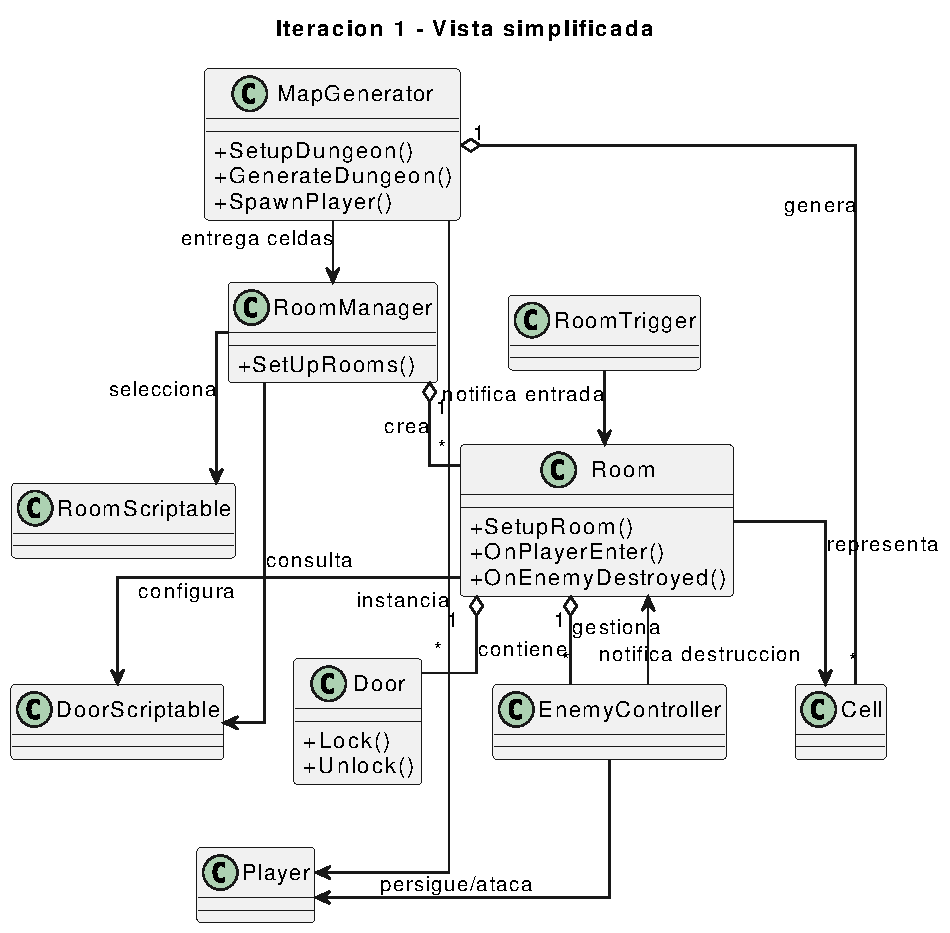
\includegraphics[width=\textwidth]{figures/iteracion1_resultado_uml.pdf}
\caption{Diagrama UML de resultado de la iteración 1}
\label{fig:uml-resultado-iteracion1}
\end{center}
\end{figure}
